% Book pp. 82-8x (PDF pp. 83-8x)
\section{Solving Real-Life Problems Involving Quadratic Inequalities}

Quadratic inequalities are a powerful tool used to model and solve various real-world
problems that involve limits, boundaries, or optimisation of quantities.
These inequalities describe relationships where one side of the equation is a
quadratic expression and are used in situations where the possible outcomes form
a range or region rather than a single point.

By learning how to solve quadratic inequalities, we can:
\begin{enumerate}
  \item Predict outcomes that must fall within thresholds like safety limits, financial
  losses, etc.
  \item Identify ranges of values that satisfy conditions in optimisation problems
  such as finding the most efficient design.
  \item Understand the critical points where changes in conditions occur, allowing
  for better decision-making and problem-solving.
\end{enumerate}
Let's go through these examples to see how the concept of quadratic inequalities
is useful in real-life.

\begin{example}{Example 2.21}
An artist is planning an art exhibition and needs to create rectangular canvases
with a specific aesthetic balance.

The total area available for displaying the artworks is limited to 80 square feet.
The artist wants the length of each canvas to be 2 feet less than its width.

To ensure that the artworks are visually appealing and fit within the assigned
space, determine the maximum width for each canvas such that the total area used
does not exceed 80 square feet.

\solution
\textbf{Step 1:} Represent the statement algebraically

Let w be the width of each canvas

Length of each canvas $=$ w $-\ 2$

\textbf{Step 2:} Write the equation for area of a rectangle

Since Area(A) $=$ width $\times$ length,

$A = w(w - 2)$

$A = w^2 - 2w$

\textbf{Step 3:} Set up the linear inequality

Since the space available for display is maximum 80 sq. feet, the total space
covered by the art can be less or equal to 80 square feet.

width $\times$ length $\le 80$

\textbf{Step 4:} Set up the quadratic inequality and simplify.
\begin{align*}
  w^2 - 2w &\le 80 \\
  w^2 - 2w - 80 &\le 0 \\
  (w - 10)(w + 8) &\le 0 \text{ (Sketch the inequality to confirm the required values)} \\
  \therefore -8 \le w &\le 10
\end{align*}
Since width can only be positive, the width of each canvas must be less than or
equal to 10 feet.

\textbf{Step 6:} State your conclusion

The artist can create canvases with a width up to 10 feet, ensuring the canvases fit
within the available display area at the exhibition.
\booknote{the book goes from Step 4 to Step 6; there is no Step 5.}
\end{example}

\begin{example}{Example 2.22}
Millicent would like to design a necklace for her mother and decides it should
resemble an eye. She makes a drawing as shown in Figure. 2.12. Identify the
systems of quadratic inequalities that helped her draw the necklace.
\begin{center}
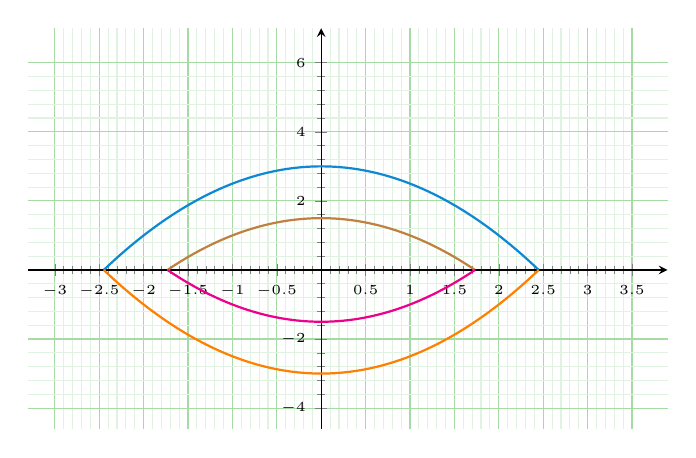
\begin{tikzpicture}
\begin{axis}[
  width=0.8\linewidth, height=0.55\linewidth,
  axis lines=middle, grid=both, minor tick num=4,
  grid style={green!60!black!35}, minor grid style={green!60!black!12},
  xmin=-3.3, xmax=3.9, ymin=-4.6, ymax=7,
  xtick={-3,-2.5,...,3.5}, ytick={-4,-2,...,6},
  tick label style={font=\tiny},
  x tick label style={/pgf/number format/fixed}
]
\addplot[cyan!70!blue, thick, domain=-2.449:2.449, samples=80] {-0.5*x^2 + 3};
\addplot[brown, thick, domain=-1.732:1.732, samples=80] {-0.5*x^2 + 1.5};
\addplot[magenta, thick, domain=-1.732:1.732, samples=80] {0.5*x^2 - 1.5};
\addplot[orange, thick, domain=-2.449:2.449, samples=80] {0.5*x^2 - 3};
\end{axis}
\end{tikzpicture}
\end{center}
\figcaption{2.12}{Necklace design}

\solution
The blue quadratic inequality curve was drawn with $y \le -0.5x^2 + 3$

The brown quadratic inequality curve was drawn with $y \ge -0.5x^2 + 1.5$

The magenta quadratic inequality curve was drawn with $y \le 0.5x^2 - 1.5$

The orange quadratic inequality curve was drawn with $y \ge 0.5x^2 - 3$
\end{example}

\begin{activity}{Activity 2.9 -- Research a Real-Life Problem}
\begin{enumerate}
  \item Identify a real-world scenario where quadratic inequalities can be
  applied. Use any of the following themes to base your research on:
  \begin{enumerate}
    \item[a.] \textbf{Agriculture:} Maximising the area of a crop field, given constraints
    such as fencing materials.
    \item[b.] \textbf{Sports:} Determining the best angle and force to kick a ball in
    football for a successful shot.
    \item[c.] \textbf{Architecture:} Designing the maximum height of an arch or
    doorway while ensuring structural safety.
    \item[d.] \textbf{Business:} Managing production costs to ensure profit margins
    while minimising loss, such as determining the optimal number
    of products to produce.
    \item[e.] \textbf{Physics:} Understanding projectile motion when an object is
    thrown into the air.
  \end{enumerate}
  \item Research how quadratic functions and inequalities play a role in this
  real-world context. Use reliable online sources, textbooks, or interview
  experts if possible.
  \item Once you've chosen your problem, model it using a quadratic inequality.

  Identify the variables in your scenario (e.g., height, distance, time, cost)
  and set up the quadratic inequality that best represents the situation.
  \item Solve the quadratic inequality you have written. Use algebraic methods
  or graphical tools to determine the solution set. You can use graphing
  software, calculators, or sketch graphs by hand to visualise the solution.
  \item Discuss the real-life implications of your solution.
  \begin{enumerate}
    \item[a.] What do the solutions of the quadratic inequality mean in terms of
    the real-world problem?
    \item[b.] What decisions can be made based on your results?
  \end{enumerate}
  \item Create a visual presentation of your findings to share with your classmates
  or teacher. Your presentation should include:
  \begin{enumerate}
    \item[a.] The real-world problem you chose.
    \item[b.] The quadratic inequality you modelled from the problem.
    \item[c.] The steps you took to solve the inequality.
    \item[d.] The real-world interpretation of the solution.
    \item[e.] Any challenges or insights you encountered while working on this
    problem.
  \end{enumerate}
\end{enumerate}
You can create a poster, a digital slide presentation or even a short video to
present your work.
\end{activity}

\section*{Extended Reading}
\begin{itemize}
  \item Baffour Ba series for schools and Colleges. (Pages 444 -- 472).
  \item Effective Elective Mathematics for Senior High School; Christian Akrong
  Hesse (Pages 202 -- 232).
  \item Effective Elective Mathematics for Senior High School, Mathematics
  Association of Ghana. (Pages 247 -- 267).
  \item Talbert, J. F., \& Heng, H. H. (1995). \textit{Additional Mathematics: Pure \&
  Applied}. Pearson Education South Asia. Page(s) 90 -- 98.
\end{itemize}
